
Unitary Fermi gas provides a curious case of a strongly-correlated many-body
quantum system where interactions are strong, but all properties of the gas are
interaction-independent. This is simply because (assuming s-wave scattering)
interparticle interactions are described by the so-called scattering length, 
and unitarity means that the scattering length is infinite. In this regime, all
information on the details of interactions drops out of all expressions which 
describe physical properties of the gas. From a theoretical point of view, the unitary regime controls
the crossover between Bardeen-Cooper-Schrieffer superconductor (BCS) and a Bose
gas of tight molecules (BEC). \cite{Eagles:1969, Legett:1980}. 
This way, the unitary gas model relates
to a wide range of physical systems, from lab-produced clouds of ultracold gases at
sub-microkelvin temperatures in magnetic and/or optical traps, to inner crusts of
neutron stars.

\subsubsection{Overview of the computational procedure}

The main computational workhorse of the study \cite{PRL:2006, NJP:2006} is a
Monte Carlo (MC) sampling in a space of (partially resummed) Feynman diagrams. 
(for a review see e.g. \cite{Gull:2011} and references therein). From the
practical point of view this is a Monte Carlo simulation where each elementary
move involves rank-1 updates of certain matrices with sizes of the order of up to
 a few thousand.

Extracting physical results from MC data is a three-stage process. First step is
a series of simulations of finite-size Hubbard clusters with varying temperature
and cluster size, at an approximately fixed value of the filling fraction of the lattice 
(via a fixed value of the chemical potential in the grand canonical ensemble.)

Second, these finite-size data are used for extracting the thermodynamic limit behavior
(i.e., the extrapolation to the inifinite system size) \emph{at a given filling fraction}.

Third, simulations are repeated for a series of filling fractions, and an
extrapolation is made towards the zero filling fraction, which corresponds to 
the continuum limit of the lattice model.

The computational complexity of a single MC simulation is, strictly speaking,
only polynomial: $O(N^3)$ for producing a single independent MC sample. Here $N$ is
proportional to the number of particles in a finite-size system, and the extrapolation
is done towards the $N\to\infty$ limit. In practice, several hundred particles are
enough to extract the thermodynamic limit.
The total simulations in 2006 took several million CPU hours on a vector Cray X1 machine.
Due to the nature of the computations (the bottleneck being
\texttt{BLAS} level 2  outer products , \texttt{dger}), the vector architecture was
extremely beneficial for larger system sizes where the performance of the 
conventional cache-based CPUs is limited by the cache size effects.

\subsubsection{Pre-replication survey: available materials}
The original work is published in a short Letter, Ref.\ \cite{PRL:2006} and
a longer, detailed paper, Ref.\ \cite{NJP:2006}.

I managed to find a backup on an old hard drive. In this archive, 
there is a folder named \texttt{code} with some 30 versions,
consistently named in a pattern \texttt{mon-date}. (Source control? Never
heard of it.) Sadly, the year did not make it into the naming scheme, and the
development was spread over at least one New Year. 
Various files have helpful ``notes-to-self'' type comments
about subtle algorithmic  tweaks and bugs, fixed or found. I am sure these
comments were very helpful back in 2006. 
One day I am going to use this as an intro slide for the
``source control considered a must'' undergraduate research skills class.

The backup archive also contains raw input/output of various simulations, and
a collection of text files with values of physical parameters, which have
probably been extracted manually from the output files. There is no versioning,
and some information can be guessed from the naming schemes of various files
and directories. 

Luckily, a website, Ref.\ \cite{MCWA}, was set up under (I believe) ``outreach and
dissemination'' rubric, and contains live demos of several
Monte Carlo codes --- and MC codes themselves! --- from the UMASS/CUNY research group. 
The website looks and feels just like one would expect from a website from 2006.
It hardly received any maintenance ever, but, remarkably, 
\emph{it still works} as of April 2020. 

The demo version downloaded from \cite{MCWA} differs from the production code
in that it is extensively commented. Combined with the paper, Ref.\ \cite{NJP:2006}
it actually allows to reconstruct the full picture with reasonable effort.
The rest of the paper attempts to document the process. 


\subsubsection{Setting up the replication exercise}

Redoing the full study, all three stages of it, is not really viable:
it is difficult to justify the use of this much CPU time. Therefore, I resorted
to reproducing a single set of steps 1 and 2 above, i.e. reproducing the
extraction of thermodynamic limit behavior at a single value of the filling
fraction. Specifically, the scope of the exercise is set to reproduce Fig.\ 2
of Ref.\ \cite{PRL:2006} (resp, Fig.\ 4 of Ref.\ \cite{NJP:2006}), which is
meant to display a ``typical'' process. 

I also decided to not use or read the raw MC data files: I will try to 
compile the code, run it, analyze the results and compare to the result
for the critical temperature, reported in Fig.\ 4 of Ref.\ \cite{NJP:2006}.
 

\subsubsection{Compiling the source code}

Compiling the code turned out to be very straightforward, even if the original did not
have a Makefile. The source is essentially a three-file Fortran 90 piece,
the only external dependency is \texttt{LAPACK}, and even the random number generator
is vendored. The code was developed with Compaq Visual Fortran on a Windows XP
desktop. There was no unit testing, but multiple runs were cross-checked on several Beowulf
clusters of AMD Opteron machines (at UMASS Amherst and ETH Zurich), and on a vector
Cray X1 machine. 

For this replication work, compilation and sample runs on today's machines: an
Ubuntu Xenial laptop with gfortran 5.4.0 with stock distro ATLAS,
and HSE HPC facilities (CentOS 7.6.1810, Intel Xeon Gold 6152
processors; Intel Parallel Studtio 2020) produce sensible results and agree with
small-scale benchmarks provided in Ref.\ \cite{MCWA}. 

Essentially, backwards compatibility is not a concern here.

\subsubsection{Using the code}

Now that the code compiles, the next step is to figure out the input and output
formats. The input is in a text file, the format is reasonably well documented
in \cite{MCWA}, and the meaning of most parameters can be traced using the 
original paper \cite{NJP:2006}. The outputs are completely undocumented, so the
only way to decipher them is to read the Fortran source. None
of the outputs (diagnostics, checkpoints, MC statistics) is versioned.

Parallelization: Monte Carlo simulations are embarassingly parallel. 
One starts a set of independent processes and 
combines the statistics in the postprocessing step. The implementation uses MPI
to start these independent MC processes with random seeds which are manually 
entered in in the parameter file
In the newer iterations of this code, the MPI part was replaced by shell
scripting, but for this exercise I am using the original code with all its warts.

For postprocessing, there is a little Fortran utility program which reads in
the data files and combines the statistics. Since data files are unversioned,
the utility must be carefully checked to be in sync with the code which wrote
the data files. 
This utility was missing from Ref.\ \cite{MCWA}, but I found it in the backups.
Otherwise, it would be possible to code it up again.  
It is included in \cite{GH:2020}.


\subsubsection{Managing the workflow}

Typical runs involve 4 to 32 independent processes for each set of physical
parameters which only differ in the value of the random seed. Running these
processes on a computing cluster is done through a batch queueing system
(SLURM or simular). Batch queueing scripts are fairly standard, and need to be
tailored to the specific configuration of each computing cluster.

Containerization (via Docker or Singularity etc) seems fashionable these days
but I decided against it since this exercise does not pose a problem containers
aim to solve (i.e., deep and fragile software stacks). 

I started with small-scale single-processor runs. A minimum reasonable run time
for a non-toy example is several CPU hours. The main hurdle for making the code
produce sensible results is instrumental parameters which control the sampling
efficiency via the size of the trial moves of the Metropolis
algorithm. If the moves are too large, they are not accepted; if they are too small,
autocorrelation times grow large. 

First several runs were producing complete bogus
because these instrumental parameters were set in \cite{MCWA} for a toy example,
and were not suitable for production runs (meaning: they would have still
have produced correct results --- in the infinite time limit only). 
Tuning these parameters is a trial and error procedure, and luckily rather coarse
tuning to reasonable values is sufficient. 

The diagnostics for this tuning is (I am writing this for the future self doing
the next replication in ten more years):

\begin{itemize}
\item The acceptance rates of the MC moves should not be outlandishly small or
too close to unity.

\item The ratio of time the simulation spends in the Green function sector and
in the Z sector must be neither too small nor too large.

\item The distribution of the diagram orders should be reasonably Gaussian-shaped,
as promised by the Central Limit Theorem (see Fig.\ \ref{fig:nmnm}).
Multiple peaks or broad shoulders signal the lack of convergence. If these are seen,
one likely needs to throw away the MC statistics and restart from a checkpointed
MC configuration.
\end{itemize}

\begin{figure}
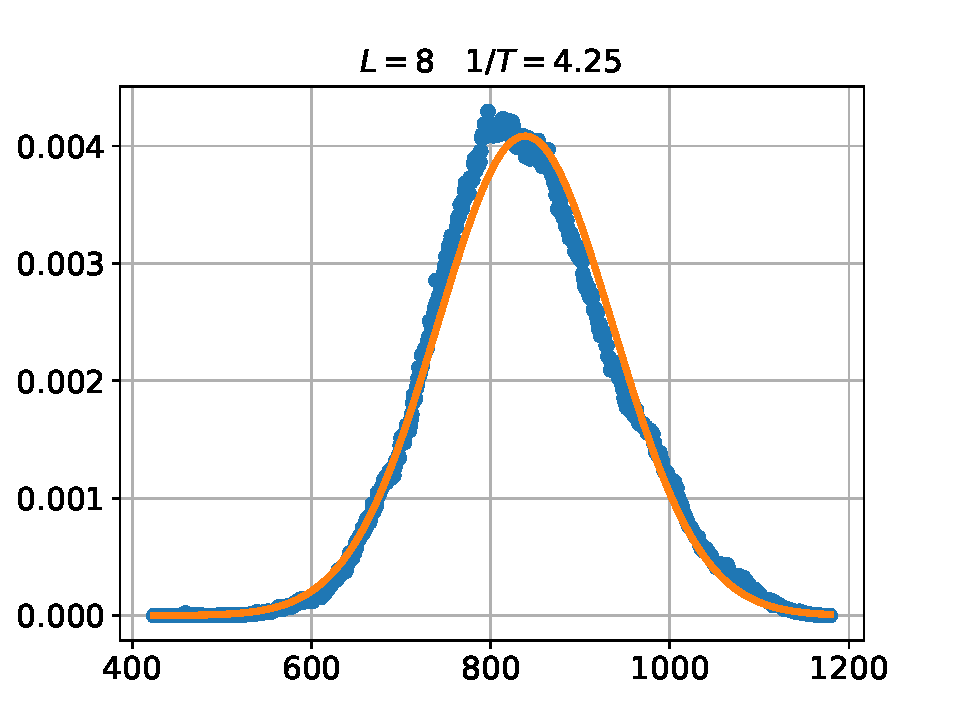
\includegraphics[width=0.49\textwidth, keepaspectratio=True]{nmnm_m52L8b425.pdf}
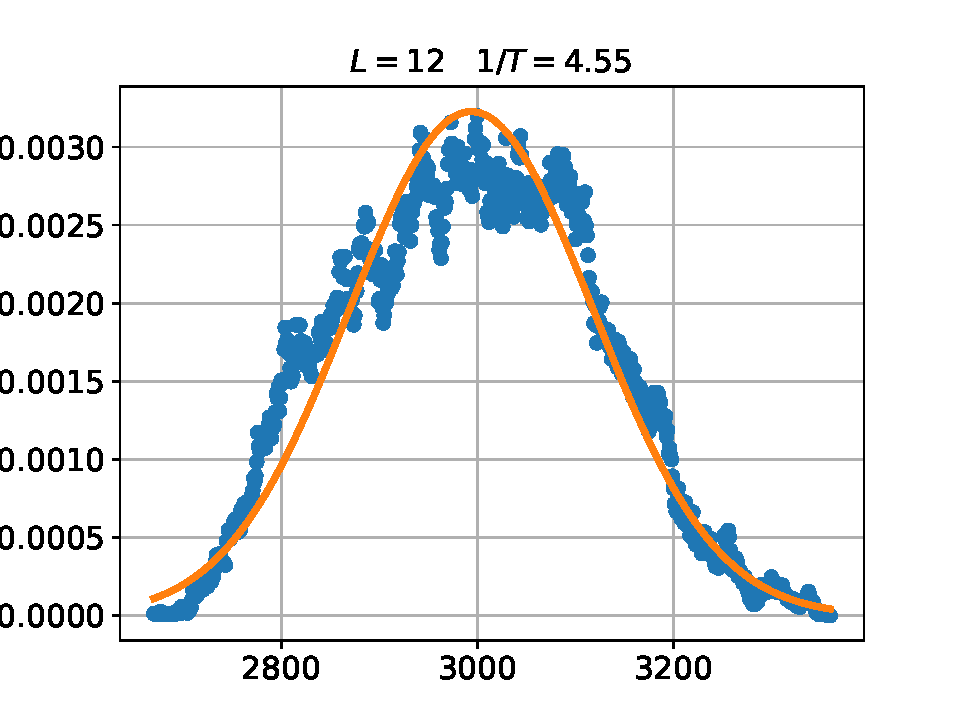
\includegraphics[width=0.49\textwidth, keepaspectratio=True]{nmnm_m52L12b455.pdf}
%
\caption{Distributions of the diagram order. Left panel: $L=8$, $1/T = 4.25$.
Right panel: $L=12$, $1/T = 4.55$. Blue points are MC results, solid lines
are gaussian shaped curves with two first moments derived from the MC data.
If a distribution is sufficiently non-gaussian (heavy tails, shoulders,
multiple peaks), it signals that the MC process has not converged. See the text
for discussion.
\label{fig:nmnm}
}
\end{figure}



\subsubsection{Data analysis}

To extract the critical temperature of the phase transition, $T_c$, from the Monte Carlo
data one uses the so-called finite size scaling: one constructs the quantity which
is scale invaritant at $T = T_c$, and fits the finite size MC data to the scaling
Ansatz using critical exponents which are fixed by the universality class.
Because of computational complexity, the available system sizes are rather small,
and thus corrections to scaling are non-negligible and need to be accounted for
in the fitting procedure. (see Sec 4 of Ref \cite{NJP:2006} for a detailed discussion).
Specifically, for $|T - T_c| \ll T_c$, the scaling Ansatz can be written as

\begin{equation}
R(L, T) = \left(f_0 + f_1 (T-T_c) L^{1/\nu} \right) \left(1 + c L^{-\omega} \right) \;,
\label{scaling}
\end{equation}
%
where $L$ is the linear size of the Hubbard cluster, $T$ is the temperature, 
$R$ is the suitably rescaled integrated pair correlator. $\nu$ and $\omega$
are critical exponents, with values $\nu \approx 0.67$ and
$\omega \approx 0.8$ for the $U(1)$ universality class. $f_0$, $f_1$ and $c$
are non-universal amplitudes. Note that if corrections-to-scaling were negligible,
$c = 0$, the curves of $R(L, T)$ versus $T$ for different $L$ would intersect at 
$T = T_c$. For system sizes which are available for simulations,
corrections-to-scaling are clearly visible, see Fig.\ \ref{fig:crossing}.

Ref.\ \cite{PRL:2006} employed a two-step procedure for extracting $T_c$ via
\eqref{scaling} where one fits a series of pairwise crossings of $R(L, T)$ curves
for pairs of $L$ values. In this work, we follow Ref.\ \cite{Goulko:2010} instead
and use Eq.\ \eqref{scaling} directly as a two-dimensional fit function
of $L$ and $T$ with four parameters, $f_0$, $f_1$, $c$ and $T_c$ (of which only
$T_c$ is of interest).


In the original work, fitting was done with the Origin point-and-click
data analysis software. Since I do not have it installed anymore, I decided
to redo the data analysis with the open source software stack
(NumPy/Scipy/Matplotlib). Ref.\ \cite{GH:2020} contains a Jupyter notebook
with full details of the data analysis. The main points are
\begin{itemize}
\item The best-fit value is $1/T_c = 4.39(5)$ which is consistent with the value
$1/T_c = 4.41(5)$ from the original work (quoted in Fig.\ 4 of Ref.\ \cite{NJP:2006})
within the combined error bars.

Note that the same data analysis with smaller MC statistics, made while
simulations were still running, (available in the git history of \cite{GH:2020})
gave a slightly different result, $1/T_c = 4.32(7)$, which is also consistent
with the original result within the combined error bars.


\item Eq.\ \eqref{scaling} is a result of linearization, which is only valid
sufficiently close to the critical point. Therefore, it is necessary to discard from
fitting the data points which are outside of a window around the $T_c$. We checked
(see \cite{GH:2020}) that (i) including points too far from $T_c$ significantly
skews the fitting procedure, and (ii) reasonable windows produce consistent results.

\item While consistent, our results do not coincide with the historic ones. 
The discrepancy can be due to a number of reasons, the most obvious one being
a slightly different fit procedure. 

\end{itemize}

I also checked the same procedure on the historic data from the archives.
Results are also consistent, but do not exactly coincide with \cite{NJP:2006}.
(see \cite{GH:2020} for full details). 
Upon closer (visual) inspection, the archive data do not exactly correspond to 
Fig.\ 2 of \cite{PRL:2006} and Fig.\ 4 of \cite{NJP:2006}. Since the archives
are not versioned and lack any sort of metadata, it's not possible to tell
whether the difference is due to typographic errors (data in text files was
definitely entered by hand) or whether these text files were work-in-progress
and final versions were lost, or if there is some other reason. Therefore,
these text files should probably be disregarded: the main point of comparison
is between the historic and today's results, and these two are consistent within
the combined error bars.

\begin{figure}
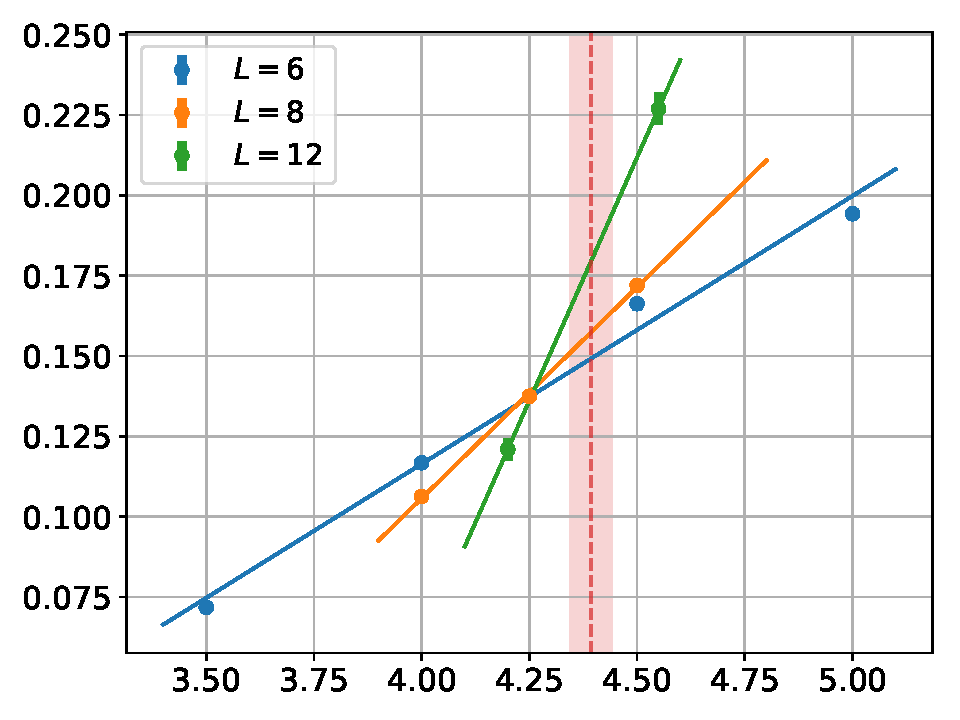
\includegraphics[width=0.49\textwidth, keepaspectratio=True]{crossing_2.pdf}
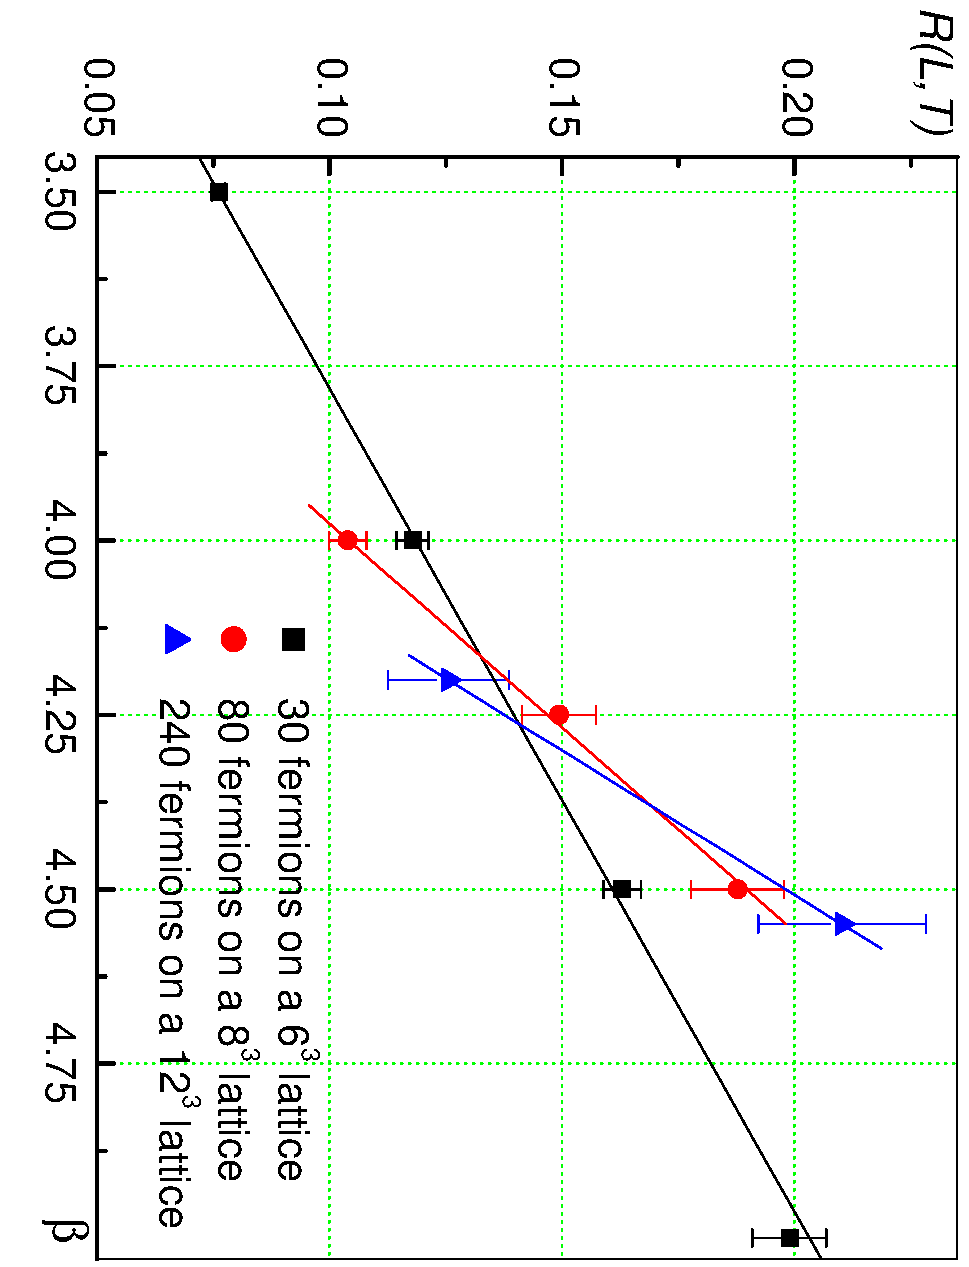
\includegraphics[width=0.47\textwidth, keepaspectratio=True]{crossing.pdf}
%
\caption{Left panel: Point: Results of MC simulations. Points are MC data with
error bars. Solid lines are linear fits to the datapoints. Red vertical line
shows the critical temperature, $1/T_c = 4.39(5)$ from the fitting procedure based
on Eq.\ \eqref{scaling}. See the text for discussion.
 Right panel: Original data and analysis. Reproduced
verbatim from Ref.\ \cite{PRL:2006}. Note that error bars are $2\sigma$ on this
panel.
\label{fig:crossing}
}
\end{figure}



\subsubsection{Conclusions and Outlook}

This work started as an exercise of reproducing a fifteen-year old computation,
and has a happy ending: results are consistent if not identical. So there is no
need to consider retracting the original paper.

The story is somewhat mundane: there is no soldering work; there is no
setting up software emulators of obsolete systems; 
there are no obscure compiler bugs to work around or undo workarounds of;
there is no wading through a brittle mess of incompatible versions of dependencies;
and there is even no need to peel through the combined mass of 
slight backwards incompatibilities which accumulates over the years.

The story here is about reproducing the workflow. Specifically, it is mostly
about tiny details which do not end up in usual artifacts (papers and even code).
The knee-jerk answer to the workflow problem is to employ a workflow and
provenance management system, and there are plenty of them over on the market.

Upon completion of this exercise, I do not believe such system would be helpful
here. First, a provenance management is code (plus dependencies!) which would need to
be audited/troubleshoot at replication time.
Second, while many workflow details can and should be automated, the main ones
still require a human being. 

Therefore, if we accept that replication is a task that cannot be fully automated,
most helpful is plain old documentation of the workflow, in a human-readable form.
Such documentation is best done in a mixture of natural language and pieces of
executable pseudocode.
%
\footnote{Python and Fortran come to mind as examples of this sort of
executable pseudocode, but that is an implementation detail.}
%
Where to place this sort of documentation? Supplementary materials, which
many peer-reviewed journals allow and even expect, provide a natural venue.
Otherwise, a supplement should be archived somewhere and cited in the paper itself.

For the original work, Refs.\ \cite{PRL:2006} and \cite{NJP:2006}, I tried to
provide this sort of a supplement, here and Ref.\ \cite{GH:2020}. I hope that it makes
next replication more straightforward. We will see in ten more years.


\subsubsection{Acknowledgements} This work was supported in part through
computational resources of HPC facilities at NRU HSE. I am indebted to
R.A.~Chulkevich for his expert tech support on the HPC cluster.
Partial support from NRU HSE project No 20-01-025 is gratefully acknowledged.




